
\subsection{The Theory of Hurricanes}
\label{sec:hurr-theory}

\subsubsection{Cyclogenesis}
\label{sec:cyclogenesis}
TCs are a finite amplitude instability created by
wind induced sea heat exchange (WISHE). There is
a clear separation between a tropical storm and a TC
in frequency of occurrance against maximum intensity~\cite{emanuel2005divine}.
`Cyclogenesis is one of the great mysteries of the tropical atmosphere'~\cite{emanuel2018progress};
although there is thermodynamic disequilibrium between the tropical sea
surface and the atmosphere TCs cannot spontaneously emerge. As first shown by
Gray 1975~\cite{gray1975tropical} there are
 diverse phenomena that triggered the growth of TC:

 In the North Atlantic, the primary triggers are African easterly waves (AEWs),
 that sometimes deepen into tropical depressions and then hurricanes,
 although AEWs can be poorly resolved in models~\cite{tomassini2017interaction}.
 Cyclogenesis can also be caused by a cold front that penetrates the tropics.

 There is a tropical cold bias in CMIP models~\cite{camargo2013global},
 possibly caused by the way moisture was dealt (see Seager 2019~\cite{seager2019strengthening}),
 and this may lead to the low TC bias in those models~\cite{tomassini2017interaction}.

\subsubsection{The Carnot cyclone}
\label{sec:carnot}

The TC can be idealised as a Carnot cycle as in Figure~\ref{fig:hurricane-carnot},
initially proposed Kleinschmidt,~1951~\cite{kleinschmidt1951grundlagen},
and then by Emanuel~1986~\cite{emanuel1986air, emanuel1987dependence, lilly1985steady,}.
\begin{figure}
\centering
    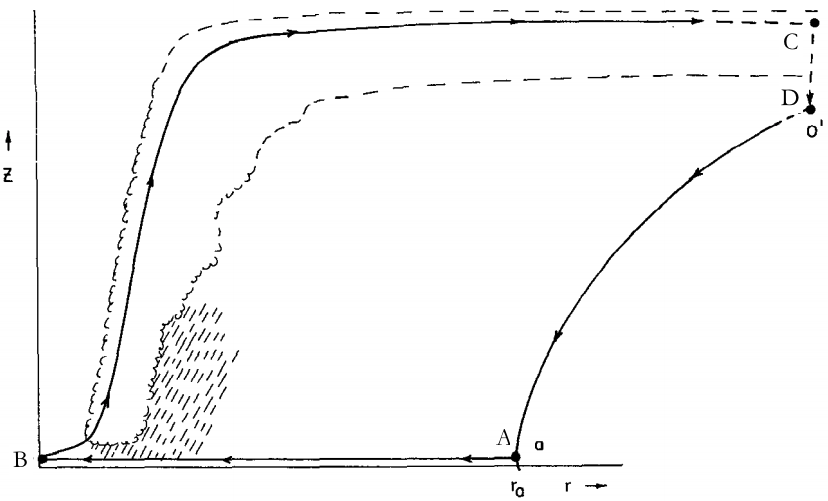
\includegraphics[width=\linewidth]{images/hurricane-carnot.png}\\
    \textit{Figure 1 from~\cite{emanuel1991theory}. }
    \caption{An idealised Carnot cycle where air parcels travel clockwise:
            A$\rightarrow$B travelling isothermally inwards into the eye-wall extracting enthalpy
            from the sea, and gaining entropy through kinetic energy dissipation;
            B$\rightarrow$C moist adiabatically thrust up into the stratosphere
            at the eye-wall and out to some some subsidence point;
            C$\rightarrow$D initial isothermal descent, albeit with some loss through radiation;
            D$\rightarrow$A final moist adiabatic descent~\cite{emanuel2018progress}. }
            \label{fig:hurricane-carnot}

\end{figure}



As shown in Figure~\ref{fig:hurricane-carnot} Enthalpy is acquired from the sea surface,
and entropy from the dissipation of kinetic energy,
 as the air travels isothermally towards the eyewall.
 At the eyewall the air rises moist adiabatically
 to the lower stratosphere and out to some distance from the storm.
 In a simplified model it then subsides
 approximately isothermally at first, albeit with some loss through radiation.
 The final descent is approximately moist adiabatic~\cite{emanuel2018progress}.

This is nearly an ideal Carnot cycle, this converts heat energy of the sea surface (see Figure~\ref{fig:heat}) into
mechanical energy of the winds, doing the majority of the work against the sea surface, where near the coast it can raise a storm surge.



\begin{figure}
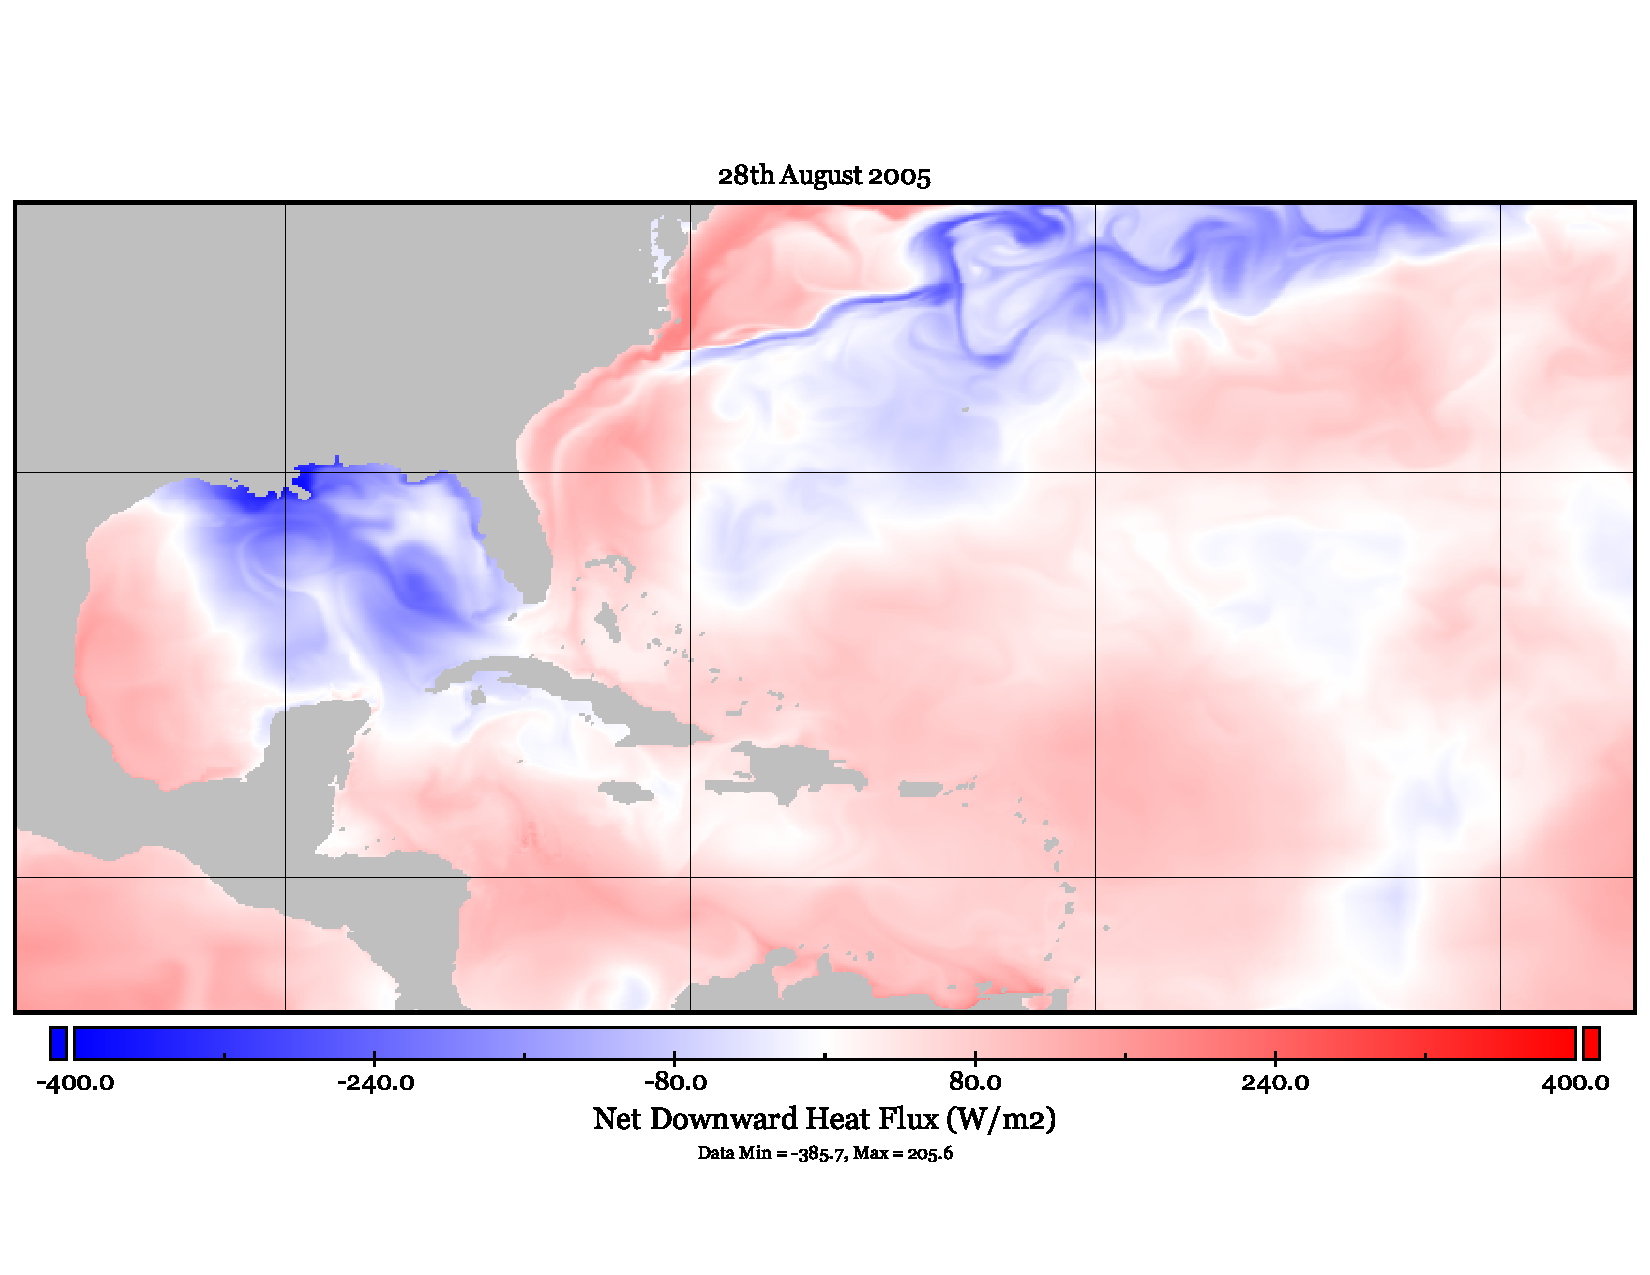
\includegraphics[width=\linewidth]{kat-heat.pdf}
\caption{The daily downwards heat flux at the sea surface on the 28th August 2005
       from \texttt{tyr}.
       The atmosphere extracts heat from the sea surface
       in the Gulf of Mexico as Katrina
       begins to make landfall. Top right shows heating of the atmosphere by
       the gulf stream (combined with an EC). }
\label{fig:heat}
\end{figure}



The potential intensity (equation 15-7 in \cite{emanuel2018progress}) is,

\begin{equation}
\left|\mathbf{V}_{s}\right|^{2}=\frac{C_{k}}{C_{D}} \frac{T_{s}-T_{o}}{T_{o}}\left(k_{0}^{*}-k\right),
\tag{PI}
\label{eq:PI}
\end{equation}

where $C_d$ is the surface drag coefficient $C_k$ is the dimensionless
surface exchange coefficient for enthalpy.
$T_s$ is the sea surface temperature ($K$), $T_o$ is the temperature of the
lower stratosphere at the end of the moist adiabatic rise ($K$).
One can see that the a warmer sea surface, and a cooler lower stratosphere
would both lead to a higher potential intensity in paragraph~\cite{emanuel1991theory, emanuel2018progress}.
Further in \ref{eq:PI} the enthalpy per unit mass (equation 15-8 in \cite{emanuel2018progress}) is

\begin{equation}
k \equiv c_{p} T+L_{v} q,
\label{eq:enthalpy_per_unit_mass}
\end{equation}

where $c_p$ is the heat capacity at constant pressure and $L_{v}$ is the latent heat
of vaporisation. $k_{0}^{*}$ is the saturation enthalpy at the sea surface~\cite{emanuel2018progress}.\footnote{
There is a positive feedback loop from air cooling adiabatically as it flows down
the pressure gradient, and therefore increasing the enthalpy disequilibrium
$k_{0}^{*}-k$, leading to a root below 700 mbar central pressure called a `hypercane'~\cite{emanuel1987dependence}
where dissipation of energy in areas apart from the sea surface must become important.

}

\begin{figure*}
\centering
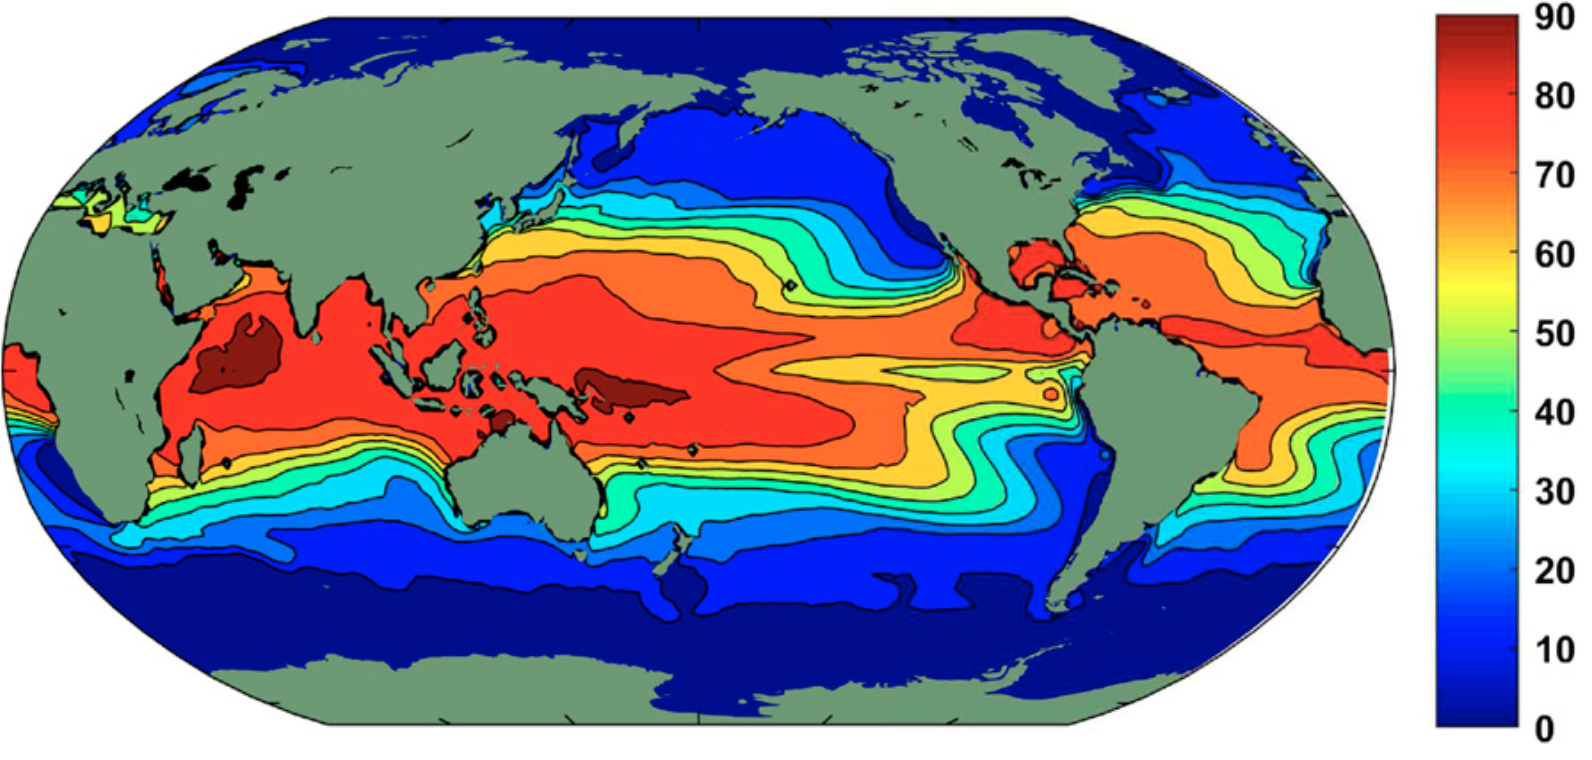
\includegraphics[width=\linewidth]{images/PI-max-year.png}\\
\textit{Figure 15-7 from \cite{emanuel2018progress}.}
\caption{The annual maximum of the potential intensity (m s$^{-1}$), calculated using
~\cite{bister2002low} and ERA-Interim data 1979-2016.
This is product maps on well to the block maxima procedure in §~\ref{sec:evt}.
}
\label{fig:eman}
\end{figure*}



Most TCs do not reach their PI. One reason for this is that not all of the
water column at the temperature
of the surface, instead only up to some depth. The majority of the cooling of
the sea surface during a TC occurs due to the
The depth of warm water
is much larger at the western boundary currents~\cite{hogg1995western}, which means that if a hurricane
travels down the axis of the current (e.g. the loop current)
it can reach a higher intensity than
if it travelled 20km to one side.


A few super-intense tropical cyclones have been observed, however the community
 trusts the assumptions made in the
Carnot cyclone model~\cite{camargo2019tropical}.
One deficiency is treating the bulk parameters
as constant (§~\ref{sec:param}).

\subsection{Contrast to extratropical cyclones}
In contrast to TCs,  ECs do not need a trigger, forming
spontaneously through the baroclinic instability
in the extratropical atmosphere~\cite{lorenz1960energy}.
ECs seem to come in a continuous spectrum.
Given that they cause significantly less damage
and smaller storm surges, and no theory has been
 set out for calculating there maximum size,
they will be largely ignored in the rest of this thesis.
